\section{User Guide:}\label{sc:userguide}

After starting the application either press the physical START button or press the on screen start button.
Now face the PS Vita toward an AR marker, once the marker is seen move the left analogue stick left and right to select the right cube to solve.
Next move the left analogue stick up and down to choose the desired face.
Once the correct cube and face is selected use the left and right shoulder buttons will rotate the selected tile left and right respectively.
To change the selected tile press the D-Pad and the selected tile will move in the same direction. 

\begin{figure}[ht!]
	\centering
	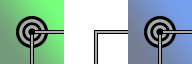
\includegraphics[width=90mm]{images/tiles.png}
	\caption{Puzzle Tiles: Left - Start, Centre - Normal, Right - End}
	\label{fig:tiles}
\end{figure}

To complete a puzzle rotate each of the tiles until there is a path from the start tile, as shown in Figure \ref{fig:tiles} as the tile with the green background, to all the end tiles, shown with a blue background.
The centre tile are plain tiles that are used as connectors.
The tiles shown are just one variation of each of the three types of tiles.
Once a puzzle is completed press either the on screen solve button or the SELECT button, this will check to see if there is a path between the start tile and all the end tiles.
If there is then the face will disappear and the next face will be selected. 

Once a cube is completed find another marker and select that cube to be solved.
When every cube has been completed the game is over.
The goal is to complete the game as quickly as possible whilst using the smallest number of solves possible.
While playing the game pressing the on screen pause button or the START button will pause the game.